% Chapter Template

\chapter{Validación y Verificación} % Main chapter title
% cSpell:disable
\label{Chapter5} % Change X to a consecutive number; for referencing this chapter elsewhere, use \ref{ChapterX}

% cSpell:enable
% cSpell:words resizebox \textit{onosapi} usecase Mcast enrutamiento parencite includegraphics pcktprocactiv lstlisting createmcast ssmprotocol

En el capítulo anterior se explicó y caracterizó el diseño de las diferentes aplicaciones que conforman el sistema. A fines de validar su funcionamiento, será necesario poner a prueba los requerimientos de cada una de las aplicaciones desarrolladas. 

De esta forma, este capítulo propone una serie de casos de prueba determinantes para verificar el funcionamiento del proyecto. 

En primer lugar, se pondrá a prueba el agente Yuma123 instalado en el dispositivo. Luego, se verifica el funcionamiento del \textit{driver} desarrollado en el controlador \textit{ONOS}. Por último, se pone a prueba tanto la interfaz \textit{REST} como la interfaz gráfica desarrollada.

%----------------------------------------------------------------------------------------
%	SECTION 1
%----------------------------------------------------------------------------------------

\section{Verificación del agente \textit{NETCONF}}

En esta sección se pondrá a prueba el agente que se instaló en el dispositivo. Para ello, las evaluaciones realizadas tendrán como objetivo asegurar el cumplimiento de los requerimientos vistos en la figura \ref{fig:req_netconf}.

\subsection{Escenario}

La figura \ref{fig:test_topo_netconf} muestra la topología utilizada para las pruebas. Se tendrá una computadora de propósito general conectada a la interfaz de control del \textit{muxponder}. Por otra parte, el \textit{muxponder} ejecutará el agente 'netconfd' de Yuma123 mientras que el \textit{host} ejecutará el cliente 'yangcli', también de Yuma123.

\begin{figure}[!h]
	\centering
	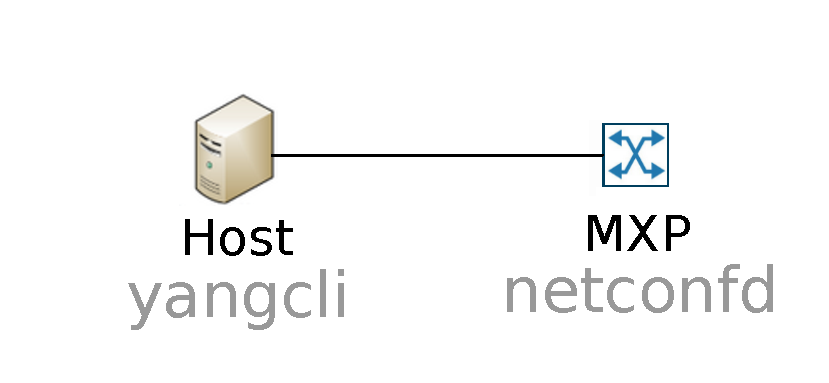
\includegraphics[scale=0.8]{Figures/topologiatestnetconf.pdf}
	\caption{Topología utilizada para las pruebas relativas a la integración del protocolo \textit{NETCONF}.}
	\label{fig:test_topo_netconf}
  \end{figure}

  \newpage

Además, para poder poner a prueba la integración del protocolo con el dispositivo se realizan las siguientes suposiciones y condiciones previas:

\begin{itemize}
	\item El \textit{host} y el \textit{muxponder} deben tener conectividad entre sí.
    \item Se debe tener instalado en el \textit{host}, el cliente 'yangcli'.
    \item Tener instalado en el \textit{muxponder}, el agente 'netconfd'.
    \item Tanto el módulo \textit{YANG} como la librería desarrollada para el \textit{muxponder}, deben estar instalados en el mismo.
    \item La aplicación 'monitor' debe estar iniciada en el \textit{muxponder}.
    \item El equipo no debe tener ninguna configuración previa aplicada.
\end{itemize}

\subsection{Matriz de trazabilidad}

Se conformarán tres casos de pruebas. El primero tiene como objetivo verificar el inicio de sesión entre el cliente y el servidor \textit{NETCONF}. Por otra parte, la segunda prueba consiste en obtener el valor de cualquier variable visible en 'monitor'. Por último, se pone a prueba realizar un cambio en la configuración del equipo.

De esta forma, la matriz de trazabilidad resultante es la que se observa en el cuadro \ref{tab:matriz_netconf}.

\begin{table}[!h]
    \centering
    \begin{tabular}{|c|c|c|c|}
    \hline
                  & \textbf{T-R-01} & \textbf{T-R-02} & \textbf{T-R-03} \\ \hline
    \textbf{R-07} & \textit{X}      & \textit{X}      & \textit{X}      \\ \hline
    \textbf{R-08} & \textit{}       & \textit{X}      & \textit{}       \\ \hline
    \textbf{R-09} & \textit{}       & \textit{}       & \textit{X}      \\ \hline
    \textbf{R-10} & \textit{}       & \textit{}       & \textit{X}      \\ \hline
    \end{tabular}
    \caption{Matriz de trazabilidad - Verificación del protocolo \textit{NETCONF}}
    \label{tab:matriz_netconf}
\end{table}


\subsection{Casos de prueba y resultados}

A continuación, se describirán los procedimientos llevados a cabo para probar esta pieza de software. Algunos de los casos de pruebas pueden estar acompañados por imágenes para esclarecer su funcionamiento.

%----------------------------------------------------------------------------------------
\subsubsection{Caso de Prueba T-R-01}
Se pondrá a prueba el inicio de la sesión \textit{NETCONF} entre el cliente y el servidor. El cuadro \ref{tab:TR01} presenta la descripción, los procedimientos y los resultados del mismo. 

\begin{table}[H]
\rowcolors{2}{white!10!gray!80}{white!80!gray!40}
\centering
\begin{tabular}{ |m{2.5cm}|m{11cm}|  }
\hline
\multicolumn{2}{|c|}{ \textbf{ID T-R-01} } \\
\hline
\centering
\textbf{Título} & Inicio de sesión en \textit{NETCONF}. \\
\hline
\centering
\textbf{Objetivo} & Poder conectarse desde el cliente \textit{NETCONF} al servidor instalado en el \textit{muxponder}.  \\
\hline
\centering
\textbf{Procedimiento} & \begin{itemize}
  \item En el muxponder, iniciar el agente \textit{NETCONF}.   
  \item En el host, haciendo uso de la \textit{CLI} del cliente 'yangcli', indicar usuario \textit{SSH}, \textit{password}, dirección IP y puerto para iniciar sesión en el servidor \textit{NETCONF} del dispositivo.
\end{itemize}     \\
\hline
\centering
\textbf{Resultados esperados} & 
Se debe observar el proceso de intercambio de capacidades entre el cliente y el servidor. 
Una vez finalizado dicho intercambio, deben quedar habilitadas las operaciones \textit{RPC} que describe tanto el protocolo como el módulo \textit{YANG} instalado en el dispositivo.
  \\

  \hline
\centering
  \textbf{Estado}    & APROBADO  \\
\hline
\end{tabular}

\caption{Caso de Prueba T-R-01}
\label{tab:TR01}
\end{table}



%----------------------------------------------------------------------------------------
  \subsubsection{Caso de Prueba T-R-02}
  En este caso, se pone a prueba las consultas por los datos de estado y de configuración del módulo \textit{YANG}. Los procedimientos para esta prueba y sus resultados se presentan en el cuadro \ref{tab:TR02}. 

  \begin{table}[H]
    \rowcolors{2}{white!10!gray!80}{white!80!gray!40}
    \centering
    \begin{tabular}{ |m{2.5cm}|m{11cm}|  }
    \hline
    \multicolumn{2}{|c|}{ \textbf{ID T-R-02} } \\
    \hline
    \centering
    \textbf{Título} & Monitoreo de datos en \textit{NETCONF}. \\
    \hline
    \centering
    \textbf{Objetivo} & Obtener información sobre las variables de estado y de configuración del dispositivo.  \\
    \hline
    \centering
    \textbf{Procedimiento} & \begin{itemize}
      \item Iniciar sesión entre un cliente y servidor \textit{NETCONF}, tal como se describió en T-R-01.   
      \item Desde el cliente, realizar consultas con las \textit{RPC get} y \textit{get-config} al contenedor \textit{mux-state-XFP1} y \textit{mux-config} respectivamente.
    \end{itemize}     \\

    \hline
    \centering
    \textbf{Resultados esperados} & 
    El servidor deberá responder, para el primer caso, valores idénticos a los que presente el binario 'monitor' respecto al módulo XFP1. 
Para el segundo caso, el servidor deberá retornar los valores de los datos de configuración que tenga el \textit{datastore running}.
\\
    
      \hline
    \centering
      \textbf{Estado}    & APROBADO  \\
    \hline
    \end{tabular}
    
    \caption{Caso de Prueba T-R-02}
    \label{tab:TR02}
    \end{table}

  Por otra parte, la figura \ref{fig:test2_consulta} ejemplifica el resultado de una operación de consulta al \textit{container} \textit{mux-state-XFP1}, el cual contiene información de estado de dicho módulo XFP.

  \begin{figure}[H]
	\centering
	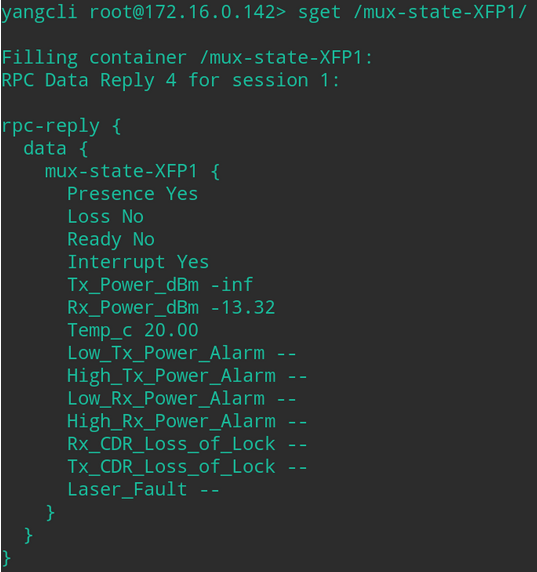
\includegraphics[scale=0.6]{Figures/test2_consulta.png}
	\caption{Consulta al \textit{container} \textit{mux-state-XFP1}.}
	\label{fig:test2_consulta}
  \end{figure}


  %----------------------------------------------------------------------------------------
  \subsubsection{Caso de Prueba T-R-03}
  Del mismo modo, el cuadro \ref{tab:TR03} detalla los procedimientos que se siguieron para verificar el funcionamiento de la  \textit{RPC} 'mux-apply-config' y las notificaciones. Cabe destacar que como se aclaró en las suposiciones para las pruebas, el equipo no se encuentra configurado. Por lo tanto se tendrán alarmas referidas a la transmisión y la recepción, entre otras. 


  \begin{table}[H]
    \rowcolors{2}{white!10!gray!80}{white!80!gray!40}
    \centering
    \begin{tabular}{ |m{2.5cm}|m{11cm}|  }
    \hline
    \multicolumn{2}{|c|}{ \textbf{ID T-R-03} } \\
    \hline
    \centering
    \textbf{Título} & Prueba de cambio de configuración y notificaciones en \textit{NETCONF}. \\
    \hline
    \centering
    \textbf{Objetivo} & Poder realizar un cambio en la configuración del dispositivo a través de la \textit{RPC} 'mux-apply-config' y verificar el funcionamiento de las notificaciones implementadas en el módulo \textit{YANG}.  \\
    \hline
    \centering
    \textbf{Procedimiento} & \begin{itemize}
      \item Iniciar sesión entre un cliente y servidor \textit{NETCONF}, tal como se describió en T-R-01.
      \item Desde el cliente \textit{NETCONF}, enviar un mensaje al servidor con la \textit{RPC} 'create-subscription'.
      \item Desde el cliente \textit{NETCONF}, enviar un mensaje al servidor con la \textit{RPC} 'mux-apply-config', para que el mismo aplique la configuración que se encuentra en el \textit{datastore running}.
    \end{itemize}     \\
    \hline
    \centering
    \textbf{Resultados esperados} & 
    En primer lugar, se espera que el cliente se suscriba correctamente a las notificaciones, recibiendo un mensaje \textit{OK} de parte del servidor. 
Además, luego de que se envíe la \textit{RPC} 'mux-apply-config' y se termine de aplicar la configuración en el equipo, en el cliente 'yangcli' se debe observar el ingreso de las notificaciones debido a que las alarmas del equipo cambiaron de estado, producto de la configuración aplicada. 
      \\
    
      \hline
    \centering
      \textbf{Estado}    & APROBADO  \\
    \hline
    \end{tabular}
    
    \caption{Caso de Prueba T-R-03}
    \label{tab:TR03}
    \end{table}


  La figura \ref{fig:test3_consulta} muestra en primer lugar cómo el cliente se suscribe a las notificaciones mediante la  \textit{RPC} 'create-suscription'. Luego, se puede observar el envío de la  \textit{RPC} 'mux-apply-config'. Seguidamente se muestran las notificaciones entrantes, producto del cambio de estado de las alarmas presentes en el equipo.
  
  \begin{figure}[H]
	\centering
	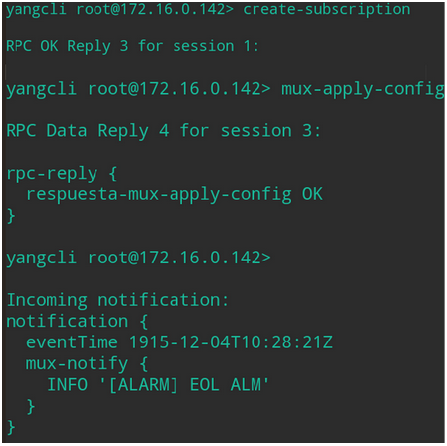
\includegraphics[scale=0.6]{Figures/test3_consulta.png}
	\caption{Suscripción y  \textit{RPC} 'mux-apply-config'.}
	\label{fig:test3_consulta}
  \end{figure}



  %----------------------------------------------------------------------------------------
%	SECTION 2
%----------------------------------------------------------------------------------------

\section{Verificación del \textit{driver}}

A continuación, en este ensayo se comprueba el funcionamiento del \textit{driver} desarrollado para el controlador \textit{ONOS}. Los requerimientos que se deben asegurar su cumplimiento son los que se observan en la figura \ref{fig:req_driver}. 

\subsection{Escenario}

En este caso, la topología utilizada para las pruebas es la que se muestra en la figura \ref{fig:test_topo_driver}. Se tendrán dos \textit{muxponders} conectados entre sí a través de las interfaces de línea de los mismos. Por otra parte, el controlador \textit{ONOS} estará conectado a la interfaz de control de ambos dispositivos. 


\begin{figure}[!h]
	\centering
	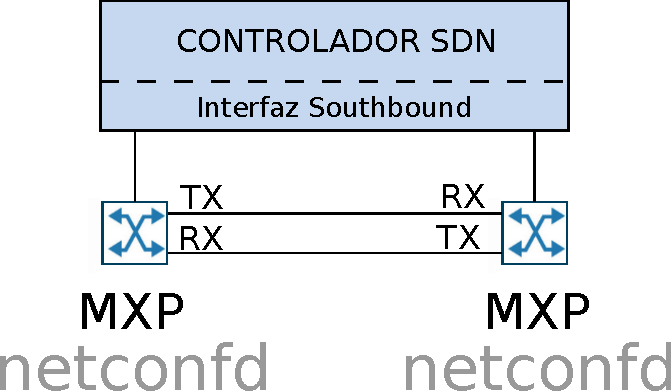
\includegraphics[scale=0.8]{Figures/topologiatestdriver.pdf}
	\caption{Topología utilizada para las pruebas relativas al \textit{driver}.}
	\label{fig:test_topo_driver}
  \end{figure}


  Además, se realizan las siguientes suposiciones:

\begin{itemize}
	\item Los agentes 'netconfd' se encuentran iniciados en ambos dispositivos.
    \item Tanto el módulo \textit{YANG} como la librería en \textit{C} desarrollada para los \textit{muxponders}, están instaladas en los mismos.
    \item La aplicación 'monitor' está iniciada en ambos \textit{muxponders}.
    \item Los dispositivos no tienen una configuración previa instalada. 
    \item Los equipos no tienen información relacionada a la presencia de vecinos.
\end{itemize}

\subsection{Matriz de trazabilidad}

A fines de poner a prueba el cumplimiento de los requerimientos para esta pieza de software, se desarrollan dos casos de prueba. 

En el primero, se verifica que el controlador sea capaz de descubrir correctamente la información de los dispositivos agregados a la topología, a través de la función \textit{DeviceDescriptionDiscovery}. La segunda prueba abarca la verificación tanto de la función \textit{LinkDiscovery} como la  \textit{RPC} 'mux-apply-config'. Además, para ambas pruebas se utilizan los comandos \textit{CLI} implementados en el \textit{driver}.

De esta forma resulta la matriz de trazabilidad que se observa en el cuadro \ref{tab:matriz_driver}.


\begin{table}[!h]
    \centering
    \begin{tabular}{|c|c|c|}
        \hline
        \textbf{}     & \textbf{T-R-04} & \textbf{T-R-05} \\ \hline
        \textbf{R-11} & \textit{X}      & \textit{}       \\ \hline
        \textbf{R-12} & \textit{}       & \textit{X}      \\ \hline
        \textbf{R-13} & \textit{}       & \textit{X}      \\ \hline
        \textbf{R-14} & \textit{X}      & \textit{X}      \\ \hline
        \end{tabular}
    \caption{Matriz de trazabilidad - Verificación del \textit{driver}}
    \label{tab:matriz_driver}
\end{table}

\subsection{Casos de prueba y resultados}

  %----------------------------------------------------------------------------------------
\subsubsection{Caso de Prueba T-R-04}

Se pondrá a prueba la función llamada \textit{DeviceDescriptionDiscovery}, la cual como se explicó en el capítulo anterior \ref{driverr}, es la encargada de registrar en el controlador información adicional de los equipos. Tanto la descripción como los procedimientos llevados a cabo y los resultados de los mismos se presentan en el cuadro \ref{tab:TR04}. 

\begin{table}[H]
  \rowcolors{2}{white!10!gray!80}{white!80!gray!40}
  \centering
  \begin{tabular}{ |m{2.5cm}|m{11cm}|  }
  \hline
  \multicolumn{2}{|c|}{ \textbf{ID T-R-04} } \\
  \hline
  \centering
  \textbf{Título} & Prueba de añadir \textit{muxponders} a la topología de ONOS.  \\
  \hline
  \centering
  \textbf{Objetivo} & Comprobar que los dispositivos se agregan correctamente al controlador, mostrando información sobre fabricante, versión del hardware y del software, identificador único, etc.  \\
  \hline
  \centering
  \textbf{Procedimiento} & \begin{itemize}
    \item Haciendo uso del comando 'onos-netcfg', enviar al controlador un mensaje \textit{JSON} con información de los dispositivos a añadir a la topología de \textit{ONOS}.
    \item Ejecutar el comando 'devices' en la \textit{CLI} del controlador. El mismo devuelve una lista con información de todos los dispositivos agregados.
  \end{itemize}     \\
  \hline
  \centering
  \textbf{Resultados esperados} & 
  Una vez que el proceso de descubrimiento de los dispositivos haya finalizado, el comando 'devices' deberá arrojar información sobre los equipos, mostrando correctamente los datos nombrados anteriormente (información del fabricante, versión de hardware y de software e identificador único).
    \\
  
    \hline
  \centering
    \textbf{Estado}    & APROBADO  \\
  \hline
  \end{tabular}
  
  \caption{Caso de Prueba T-R-04}
  \label{tab:TR04}
  \end{table}

  Por otra parte, la figura \ref{fig:test4_consulta} muestra los dispositivos agregados a la topología de \textit{ONOS}. Al hacer click sobre cualquiera de ellos, el controlador despliega un cuadro del dispositivo seleccionado mostrando la información mencionada anteriormente.

  \begin{figure}[H]
	\centering
	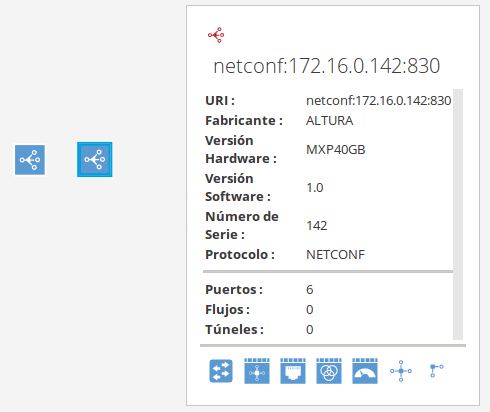
\includegraphics[scale=0.5]{Figures/test4_consulta.png}
	\caption{Información de dispositivos presentes en la topología de \textit{ONOS}.}
	\label{fig:test4_consulta}
  \end{figure}

  %----------------------------------------------------------------------------------------
  \subsubsection{Caso de Prueba T-R-05}

  Este caso pone a verifica tanto la función \textit{LinkDiscovery}, la cual es la encargada de formar los enlaces entre los distintos dispositivos \ref{driverlink}, como la  \textit{RPC} 'mux-apply-config', encargada de aplicar los cambios en el dispositivo \ref{drivermux}. 
  En el cuadro \ref{tab:TR05} se detalla la descripción del caso de prueba mencionado. Se asumirá que los dispositivos ya se encuentran añadidos al controlador.
  

  \begin{table}[H]
    \rowcolors{2}{white!10!gray!80}{white!80!gray!40}
    \centering
    \begin{tabular}{ |m{2.5cm}|m{11cm}|  }
    \hline
    \multicolumn{2}{|c|}{ \textbf{ID T-R-05} } \\
    \hline
    \centering
    \textbf{Título} & Prueba de formar enlaces entre \textit{muxponders} vecinos.  \\
    \hline
    \centering
    \textbf{Objetivo} & Comprobar que el controlador muestra correctamente la información referida a los enlaces entre los dispositivos.   \\
    \hline
    \centering
    \textbf{Procedimiento} & \begin{itemize}
      \item Desde el controlador, agregar información del vecino a cada uno de los dispositivos presentes en la topología.
      \item Haciendo uso de la \textit{RPC} 'mux-apply-config', aplicar una misma configuración a todos los equipos. 
      \item Desconectar el transmisor de alguno de los \textit{muxponders}.
    \end{itemize}     \\
    \hline
    \centering
    \textbf{Resultados esperados} & 
    Al agregar a cada dispositivo la información referente a su vecino, se deberá observar en la interfaz gráfica de \textit{ONOS} que los enlaces no se forman. Esto es así ya que como los dispositivos no están configurados, existirán alarmas referidas a la transmisión y recepción, y como se explicó en el capítulo anterior el \textit{driver} no formará los enlaces si dichas alarmas están presentes. 

Luego, al enviar la \textit{RPC} 'mux-apply-config' a ambos dispositivos y una vez que se termine de aplicar la configuración, las alarmas mencionadas anteriormente deberían desaparecer. Por lo tanto, en la interfaz gráfica del controlador se debe observar los enlaces formados entre los equipos, ya que no existen alarmas relacionadas a la transmisión y recepción.
Por último, el hecho de desconectar la línea del transmisor en alguno de los dos \textit{muxponders} genera alarmas en los dispositivos, por lo que la interfaz gráfica debe mostrar un cambio en la topología debido a que el enlace no se encuentra presente.  
      \\
    
      \hline
    \centering
      \textbf{Estado}    & APROBADO  \\
    \hline
    \end{tabular}
    
    \caption{Caso de Prueba T-R-05}
    \label{tab:TR05}
    \end{table}

  La figura \ref{fig:test5_1} muestra la topología presente en el controlador una vez se le indicó a cada dispositivo la presencia de un vecino. Como se puede notar, el controlador no forma los enlaces entre los mismos ya que los dispositivos contienen alarmas debido a que no están configurados. 

  \begin{figure}[H]
	\centering
	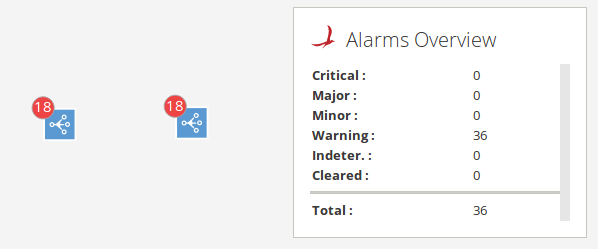
\includegraphics[scale=0.5]{Figures/test5_1.png}
	\caption{Vista de la topología de \textit{ONOS} - Dispositivos sin configurar.}
	\label{fig:test5_1}
  \end{figure}

  A su vez, en la figura \ref{fig:test5_2} se observa que una vez aplicada la configuración en ambos dispositivos, la cantidad de alarmas presentes se reducen. Luego, al no existir alarmas referidas a la transmisión y recepción de los equipos, el controlador puede formar correctamente el enlace entre los mismos. 

  \begin{figure}[H]
	\centering
	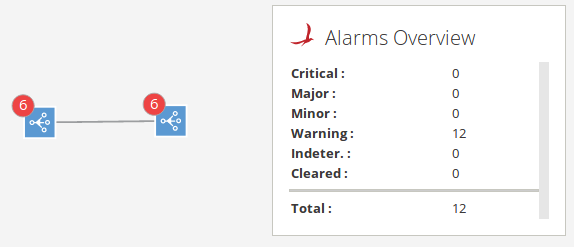
\includegraphics[scale=0.5]{Figures/test5_2.png}
	\caption{Vista de la topología de \textit{ONOS} - Dispositivos configurados.}
	\label{fig:test5_2}
  \end{figure}

  Por último, la figura \ref{fig:test5_3} ejemplifica lo que sucede cuando se desconecta el transmisor en alguno de los dispositivos, provocando así la caída de un enlace en la topología de \textit{ONOS}.

  \begin{figure}[H]
	\centering
	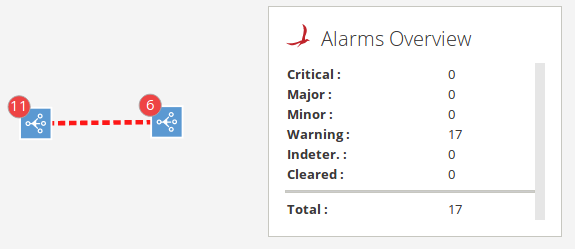
\includegraphics[scale=0.5]{Figures/test5_3.png}
	\caption{Vista de la topología de \textit{ONOS} - Dispositivos configurados, con un enlace desconectado.}
	\label{fig:test5_3}
  \end{figure}



%----------------------------------------------------------------------------------------
%	SECTION 3
%----------------------------------------------------------------------------------------

\section{Verificación de la interfaz gráfica y la interfaz \textit{REST}}

Finalmente, en esta sección se pondrán a prueba ambas interfaces desarrolladas. Para ello, las pruebas realizadas tendrán como objetivo validar el cumplimiento de los requerimientos vistos en la figura \ref{fig:req_app}. 

Además, los casos de prueba presentados a continuación harán uso tanto del \textit{driver} como de la aplicación \textit{C} desarrollada para el agente \textit{NETCONF}.


\subsection{Escenario}

La topología utilizada para las pruebas mencionadas anteriormente se muestra en la figura \ref{fig:test_topo_rest}. 
Se tendrán dos \textit{muxponders} conectados entre sí a través de las interfaces de línea de los mismos. Además, el controlador \textit{ONOS} estará conectado a la interfaz de control de ambos dispositivos. Por último, se tienen dos computadoras de propósito general conectadas a los módulos XFP1 de los \textit{muxponders}.



\begin{figure}[H]
	\centering
	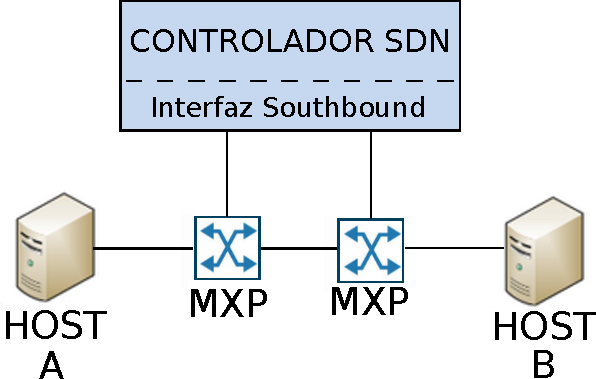
\includegraphics[scale=0.8]{Figures/topologiatest.pdf}
	\caption{Topología utilizada para las pruebas relativas a la interfaz gráfica e interfaz \textit{REST}.}
	\label{fig:test_topo_rest}
  \end{figure}


  Además, se realizan las siguientes suposiciones:

\begin{itemize}
	\item Los agentes 'netconfd' se encuentran iniciados en ambos dispositivos.
    \item Tanto el módulo \textit{YANG} como la librería en \textit{C} desarrollada para los \textit{muxponders}, están instaladas en los mismos.
    \item La aplicación 'monitor' está iniciada en ambos \textit{muxponders}.
    \item Los dispositivos no tienen una configuración previa instalada. 
    \item Los equipos no tienen información relacionada a la presencia de vecinos.
\end{itemize}


\subsection{Matriz de trazabilidad}

Se presenta a continuación en el cuadro \ref{tab:matriz_rest} la matriz de trazabilidad para las pruebas realizadas. 

En la primera prueba, se verifica poder agregar dispositivos a través de la interfaz gráfica y configurar a ambos como vecinos. 
Luego, se verifica en la prueba T-R-07 que puedan visualizarse las alarmas en la aplicación \textit{WEB}.
Por otra parte, en la prueba T-R-08 se comprueba que sea posible visualizar, a través de la interfaz gráfica, cualquier dato de estado de los dispositivos.
Por último, se ensaya realizar un cambio en la configuración en los dispositivos de tal forma que se permita la conectividad entre los \textit{host} A y B.
\\


\begin{table}[!h]
    \centering
    \begin{tabular}{|c|c|c|c|c|}
      \hline
      \textbf{}     & \textbf{T-R-06} & \textbf{T-R-07}    & \textbf{T-R-08} & \textbf{T-R-09} \\ \hline
      \textbf{R-15} & \textit{}       & \textit{X}         & \textit{X}      & \textit{X}      \\ \hline
      \textbf{R-16} & \textit{X}      & \textit{}          & \textit{}       & \textit{X}      \\ \hline
      \textbf{R-17} & \textit{}       & \textit{\textbf{}} & \textit{}       & \textit{X}      \\ \hline
      \textbf{R-18} & \textit{}       & \textit{X}         & \textit{}       & \textit{}       \\ \hline
      \textbf{R-19} & \textit{X}      & \textit{}          & \textit{}       & \textit{X}      \\ \hline
      \textbf{R-20} & \textit{}       & \textit{}          & \textit{}       & \textit{X}      \\ \hline
      \textbf{R-21} & \textit{}       & \textit{}          & \textit{X}      & \textit{}       \\ \hline
      \end{tabular}
    \caption{Matriz de trazabilidad - Verificación de la interfaz \textit{REST} e interfaz gráfica}
    \label{tab:matriz_rest}
\end{table}


\subsection{Casos de prueba y resultados}

\subsubsection{Caso de Prueba T-R-06}

A continuación, se asegura agregar nuevos dispositivos a la topología del controlador desde la interfaz gráfica y configurarlos como vecinos. Los procedimientos llevados a cabo para dicha prueba se observan en el cuadro \ref{tab:TR06}.


\begin{table}[H]
  \rowcolors{2}{white!10!gray!80}{white!80!gray!40}
  \centering
  \begin{tabular}{ |m{2.5cm}|m{11.5cm}|  }
  \hline
  \multicolumn{2}{|c|}{ \textbf{ID T-R-06} } \\
  \hline
  \centering
  \textbf{Título} & Añadir \textit{muxponders} a la topología de \textit{ONOS} desde la interfaz gráfica y configurarlos como vecinos.  \\
  \hline
  \centering
  \textbf{Objetivo} & Comprobar que los dispositivos se agregan correctamente al controlador haciendo uso de la interfaz gráfica y que es posible agregar información de vecinos a cada uno de ellos desde la misma.   \\
  \hline
  \centering
  \textbf{Procedimiento} & \begin{itemize}
    \item Desde la aplicación \textit{WEB}, agregar un nuevo dispositivo indicando dirección IP y puerto.
    \item Desde la aplicación \textit{WEB}, hacer click en 'TOPOLOGIA' y configurar ambos equipos como vecinos.
    \item En el controlador, ejecutar el comando 'devices'.
    \item Desde la aplicación \textit{WEB}, hacer click en 'CONFIGURACION'.
  \end{itemize}     \\
  \hline
  \centering
  \textbf{Resultados esperados} & 
  Luego de ejecutar el comando 'devices' en la \textit{CLI} del controlador, se debe mostrar la información de fabricante, versión del hardware y software e identificador único de ambos dispositivos agregados. 
Por otra parte, la sección 'CONFIGURACION' debe mostrar la información mencionada anteriormente junto con el identificador único del vecino agregado. 
  
    \\
  
    \hline
  \centering
    \textbf{Estado}    & APROBADO  \\
  \hline
  \end{tabular}
  
  \caption{Caso de Prueba T-R-06}
  \label{tab:TR06}
  \end{table}



  \subsubsection{Caso de Prueba T-R-07}

El objetivo del caso de prueba presentado en el cuadro \ref{tab:TR07}, es el de verificar que la interfaz gráfica presente de forma correcta la información relacionada a las alarmas en los dispositivos. 
Se hará uso tanto de la aplicación 'monitor' como de los comandos '\textit{alarms}' y '\textit{alarms-count}' de \textit{ONOS} para validar las alarmas presentes.


\begin{table}[H]
  \rowcolors{2}{white!10!gray!80}{white!80!gray!40}
  \centering
  \begin{tabular}{ |m{2.5cm}|m{11cm}|  }
  \hline
  \multicolumn{2}{|c|}{ \textbf{ID T-R-07} } \\
  \hline
  \centering
  \textbf{Título} & Prueba de visualización de alarmas desde la interfaz gráfica.  \\
  \hline
  \centering
  \textbf{Objetivo} & Comprobar que la aplicación \textit{WEB} muestra correctamente las alarmas de todos los \textit{muxponders} presentes en la topología.   \\
  \hline
  \centering
  \textbf{Procedimiento} & \begin{itemize}
    \item En la aplicación \textit{WEB}, hacer click sobre 'ALARMAS'.
    \item En el controlador, ejecutar los comandos 'alarms' y 'alarms-counts'. 
    \item En la \textit{CLI} de cada uno de los \textit{muxponders}, verificar con la aplicación 'monitor' la presencia de alarmas.
  \end{itemize}     \\
  \hline
  \centering
  \textbf{Resultados esperados} & 
  La cantidad de alarmas presentes anunciadas en la interfaz gráfica debe ser la misma que las anunciadas por el controlador al ejecutar el comando 'alarms-counts'.
Además, la información referida a cada alarma, como por ejemplo el dispositivo de origen y el nombre de la misma, debe ser igual a las que muestre el comando 'alarms' en el controlador \textit{ONOS}.
Finalmente, las alarmas presentes en cada dispositivo deben poder visualizarse en la aplicación 'monitor' de los \textit{muxponders} relacionados. 
    \\
  
    \hline
  \centering
    \textbf{Estado}    & APROBADO  \\
  \hline
  \end{tabular}
  
  \caption{Caso de Prueba T-R-07}
  \label{tab:TR07}
  \end{table}

  Tal como se puede ver en la figura \ref{fig:test7_1}, se tienen 12 alarmas presentes referidas a los módulos XFP2, XFP3 y XFP4 de ambos dispositivos.

  \begin{figure}[H]
	\centering
	\resizebox{\textwidth}{!}{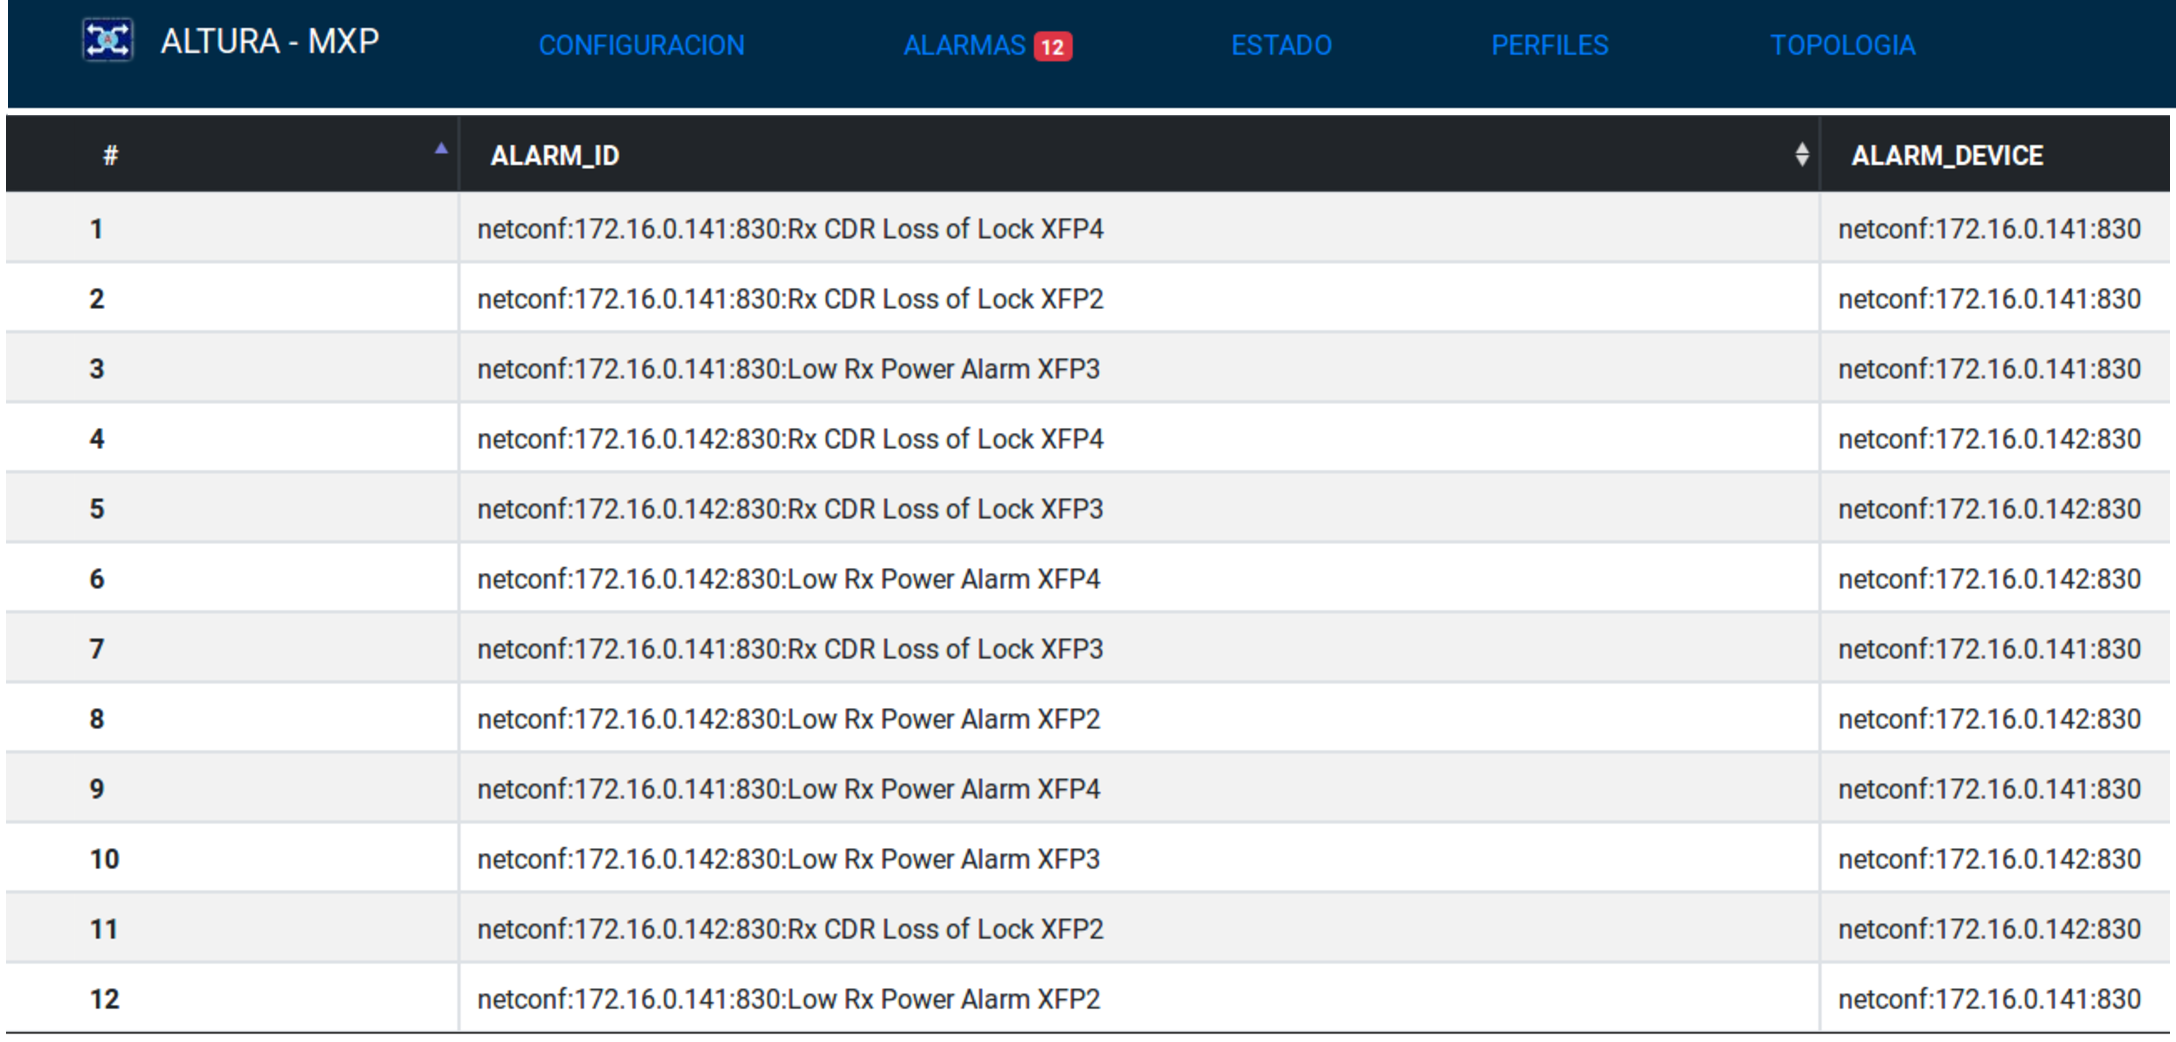
\includegraphics{Figures/test7_1.pdf}}
	\caption{Alarmas visualizadas en la interfaz gráfica.}
	\label{fig:test7_1}
  \end{figure}

  Se puede observar lo mismo al ejecutar los comandos '\textit{alarms}' y '\textit{alarms-counts}', los cuales listan las alarmas presentes en el controlador. De esta forma, se puede ver en la figura \ref{fig:test7_2} la salida del comando '\textit{alarms-counts}', la cual anuncia la misma cantidad de alarmas presentes en el controlador.

  \begin{figure}[H]
	\centering
	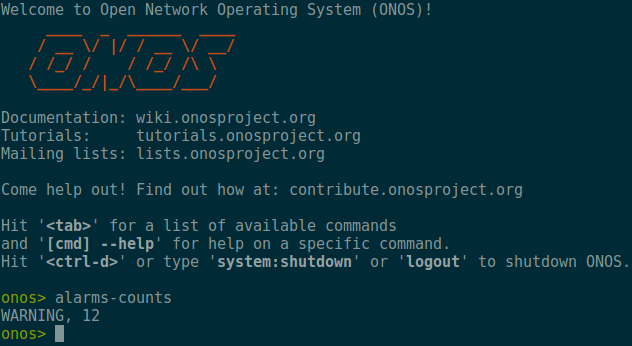
\includegraphics[scale=0.5]{Figures/test7_2.png}
	\caption{Alarmas visualizadas en la \textit{CLI} del controlador.}
	\label{fig:test7_2}
  \end{figure}

  Por último, se muestra en la figura \ref{fig:test7_3} la salida del binario 'monitor' de uno de los \textit{muxponder}. En ella, es posible observar 6 etiquetas '\textit{Alarm}' en la sección de modulos XFP. Teniendo en cuenta que se tiene el mismo resultado en el otro dispositivo, se tienen las 12 alarmas en total.

  \begin{figure}[H]
	\centering
	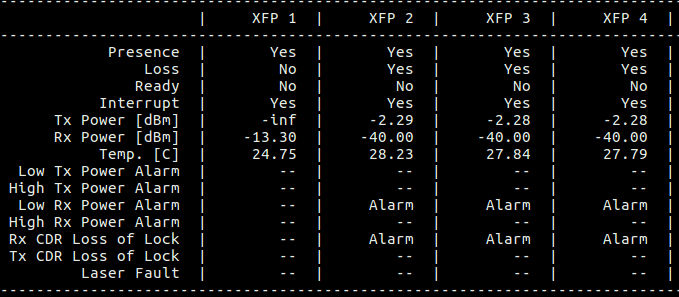
\includegraphics[scale=0.5]{Figures/test7_3.png}
	\caption{Alarmas visualizadas en 'monitor' en uno de los \textit{muxponders}.}
	\label{fig:test7_3}
  \end{figure}

  \subsubsection{Caso de Prueba T-R-08}

  Se presenta la verificación que se observa en el cuadro \ref{tab:TR08}, la cual tiene como objetivo examinar que sea posible observar cualquier dato de estado del dispositivo a través de la interfaz gráfica. 
  
  Al igual que en la prueba anterior, se hará uso del binario 'monitor' para comprobar su funcionamiento.
  
  
  \begin{table}[H]
    \rowcolors{2}{white!10!gray!80}{white!80!gray!40}
    \centering
    \begin{tabular}{ |m{2.5cm}|m{11cm}|  }
    \hline
    \multicolumn{2}{|c|}{ \textbf{ID T-R-08} } \\
    \hline
    \centering
    \textbf{Título} & Prueba de visualización de los datos de estado desde la interfaz gráfica.  \\
    \hline
    \centering
    \textbf{Objetivo} & Verificar que desde la aplicación \textit{WEB} se pueda obtener información de los datos de estado de cada \textit{muxponder} presente en la topología.   \\
    \hline
    \centering
    \textbf{Procedimiento} & \begin{itemize}
      \item En la aplicación \textit{WEB}, hacer click sobre 'ESTADO'.
      \item En el controlador, consultar por los datos de estado de cada dispositivo presente haciendo uso del comando 'get'. 
      \item Verificar con 'monitor' los valores para los datos de estado.
    \end{itemize}     \\
    \hline
    \centering
    \textbf{Resultados esperados} & 
    La información que presenta la sección 'ESTADO' de la interfaz gráfica debe tener valores idénticos a los obtenidos por el controlador luego de ejecutar el comando 'get'.

Además, la información que muestra 'monitor' debe coincidir con la que se observa en la sección de 'ESTADO' en la aplicación \textit{WEB}.
      \\
    
      \hline
    \centering
      \textbf{Estado}    & APROBADO  \\
    \hline
    \end{tabular}
    
    \caption{Caso de Prueba T-R-08}
    \label{tab:TR08}
    \end{table}

    A continuación, en la figura \ref{fig:test8_1} se muestran los valores obtenidos por la interfaz gráfica referidos al \textit{container} '\textit{misc}' de ambos dispositivos. 

    \begin{figure}[H]
        \centering
        \resizebox{\textwidth}{!}{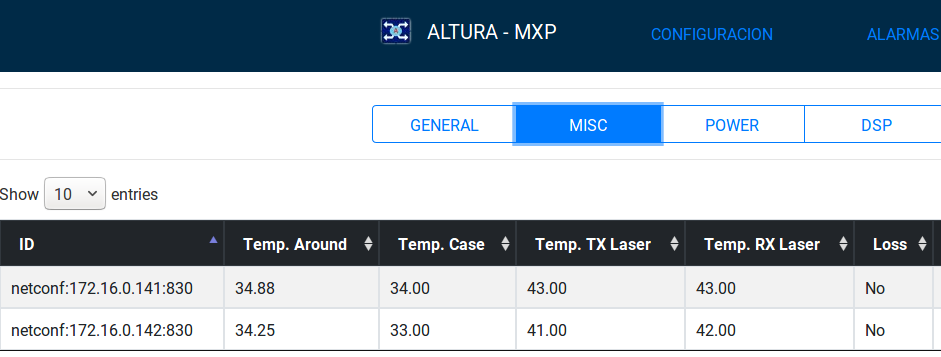
\includegraphics{Figures/test8_1.png}}
        \caption{Datos de estado, observados desde la interfaz gráfica.}
        \label{fig:test8_1}
      \end{figure}

      Por otra parte, se observa en la figura \ref{fig:test8_2} la sección referida a '\textit{misc}' en 'monitor', los cuales tienen los mismos valores que los obtenidos por la interfaz gráfica. Es importante aclarar que debido a la cantidad de los datos presentes en este \textit{container}, las figuras nombradas anteriormente solo muestran una porción de los datos.
      
      Por lo tanto, se observan únicamente los primeros cinco valores.

      \begin{figure}[H]
        \centering
        \begin{subfigure}[b]{0.45\textwidth}
            \centering
            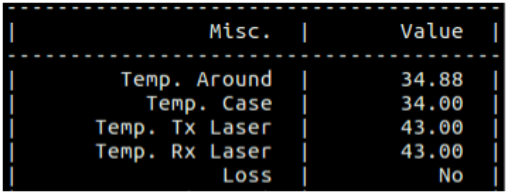
\includegraphics[width=\textwidth]{Figures/test8_2_mux1.png}
            \caption{'monitor' del \textit{muxponder} '141'.}
        \end{subfigure}
        \quad
        \begin{subfigure}[b]{0.45\textwidth}  
            \centering 
            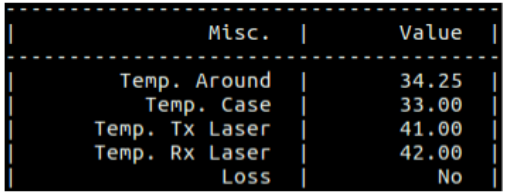
\includegraphics[width=\textwidth]{Figures/test8_2_mux2.png}
            \caption{'monitor' del \textit{muxponder} '142'.}
        \end{subfigure}
        \caption{Datos de estado, observados desde 'monitor'.}
        \label{fig:test8_2}
    \end{figure}

      \subsubsection{Caso de Prueba T-R-09}

      Por último, el caso de prueba mostrado en el cuadro \ref{tab:TR09} tiene como objetivo verificar que es posible configurar los \textit{muxponders} de tal manera que los \textit{host} A y B tengan conectividad entre sí. 

      \begin{table}[H]
        \rowcolors{2}{white!10!gray!80}{white!80!gray!40}
        \centering
        \begin{tabular}{ |m{2.5cm}|m{11cm}|  }
        \hline
        \multicolumn{2}{|c|}{ \textbf{ID T-R-09} } \\
        \hline
        \centering
        \textbf{Título} & Prueba de conectividad entre los \textit{hosts} A y B.  \\
        \hline
        \centering
        \textbf{Objetivo} & Poder configurar a través de la interfaz gráfica ambos \textit{muxponders}, con el objetivo de que los \textit{hosts} tengan conectividad entre ellos.   \\
        \hline
        \centering
        \textbf{Procedimiento} & \begin{itemize}
          \item Desde la sección 'TOPOLOGÍA' en la aplicación \textit{WEB}, configurar ambos dispositivos como vecinos.
          \item Hacer click en la sección 'PERFILES' y añadir dos perfiles, uno con tipo de tráfico 'xge' y otro con un tipo de tráfico 'otu2'.
          \item  Hacer click en 'ALTURA-MXP'. En el cuadro de configuración, aplicar a uno de los dispositivos el perfil de configuración 'xge' mientras que al otro aplicar el perfil de configuración 'otu2'.
          \item En cada uno de los \textit{hosts}, verificar si tienen conectividad entre ellos utilizando la aplicación 'ping'.
          \item Hacer click en 'CONFIGURACION'. Verificar la configuración aplicada en los dispositivos.
          \item Hacer click en 'ALTURA-MXP'. En el cuadro de configuración, seleccionar el \textit{muxponder} configurado anteriormente con el perfil 'otu2' y aplicarle ahora la configuración 'xge'.
          \item En cada uno de los \textit{hosts}, verificar si tienen conectividad entre ellos utilizando la aplicación 'ping'.

        \end{itemize}     \\
        \hline
        \centering
        \textbf{Resultados esperados} & 
        Luego de configurar a los dispositivos como vecinos y aplicar un perfil de configuración diferente a cada uno de ellos, la interfaz deberá mostrar en la sección principal una advertencia de que existen dispositivos presentes en la topología con una configuración diferente. 

        Si los \textit{muxponders} tienen aplicada una configuración diferente entre ellos, no existirá conectividad entre los host, por lo que los dispositivos no podrán realizar un 'ping' entre ellos.
 
        Luego, al configurar ambos dispositivos con el mismo perfil de configuración, la interfaz gráfica debe mostrar en la sección principal que la alarma referida a configuración inconsistente desapareció. Además, la prueba de 'ping' debe mostrar ahora que los \textit{host} pueden alcanzarse.
          \\
        
          \hline
        \centering
          \textbf{Estado}    & APROBADO  \\
        \hline
        \end{tabular}
        
        \caption{Caso de Prueba T-R-09}
        \label{tab:TR09}
        \end{table}

      La figura \ref{fig:test9_1} muestra la sección principal de la interfaz gráfica. En ella, es posible observar un recuadro en amarillo indicando que se detectó una configuración inconsistente entre los dispositivos (o sea, que los dispositivos vecinos no tienen la misma configuración). 

      \begin{figure}[H]
        \centering
        \resizebox{\textwidth}{!}{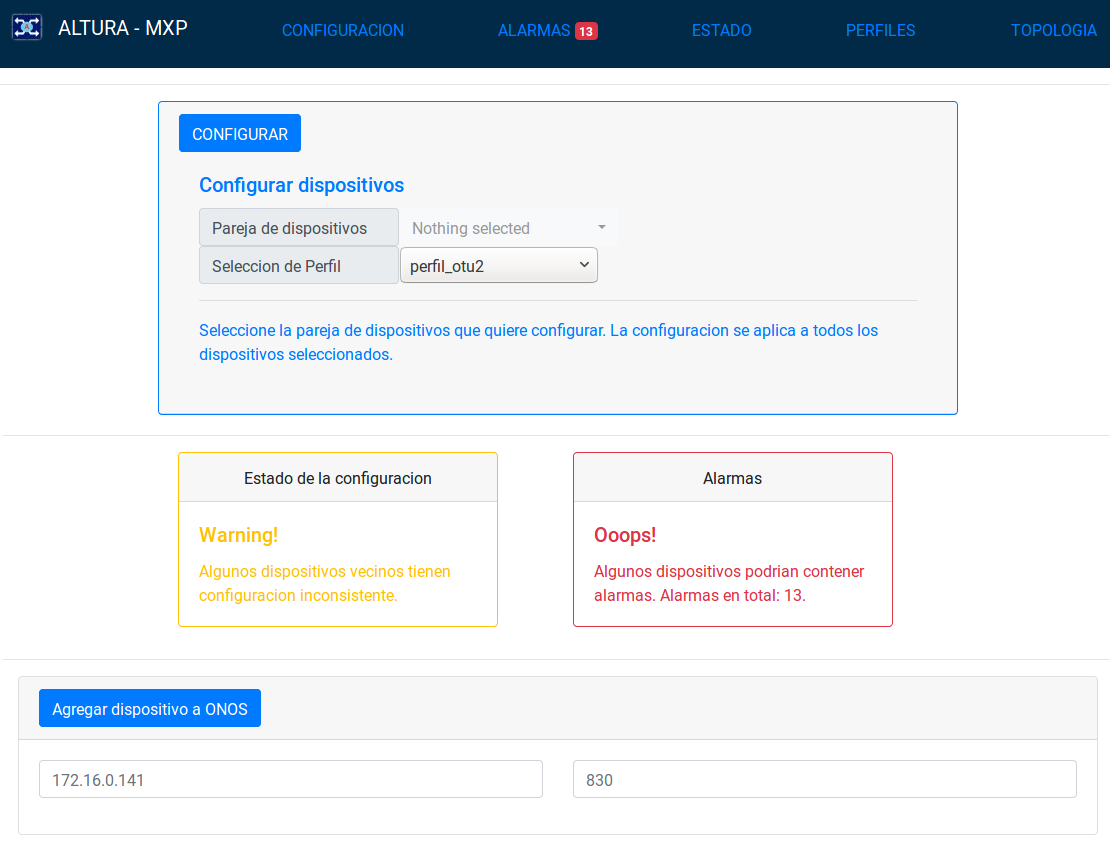
\includegraphics{Figures/test9_1.png}}
        \caption{Detección de configuración inconsistente entre dispositivos vecinos.}
        \label{fig:test9_1}
      \end{figure}

      En este estado, si los \textit{host} A y B tratan de realizar un ping entre ellos el resultado es el que se puede ver en la figura \ref{fig:test9_2}. Como se esperaba, los \textit{hosts} no tienen conectividad entre ellos debido a la configuración inconsistente aplicada a los dispositivos.

      \begin{figure}[H]
        \centering
        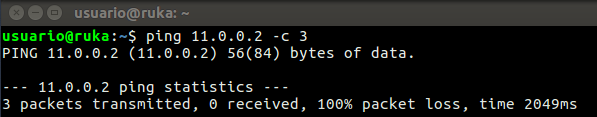
\includegraphics[scale=0.7]{Figures/test9_2.png}
        \caption{Prueba fallida de conectividad entre \textit{host} A y \textit{host} B.}
        \label{fig:test9_2}
      \end{figure}

      Luego, al configurar ambos dispositivos con el perfil de configuración xge, la interfaz muestra que la alarma debido a configuración inconsistente desapareció, tal como se muestra en la figura \ref{fig:test9_3}.


      \begin{figure}[H]
        \centering
        \resizebox{\textwidth}{!}{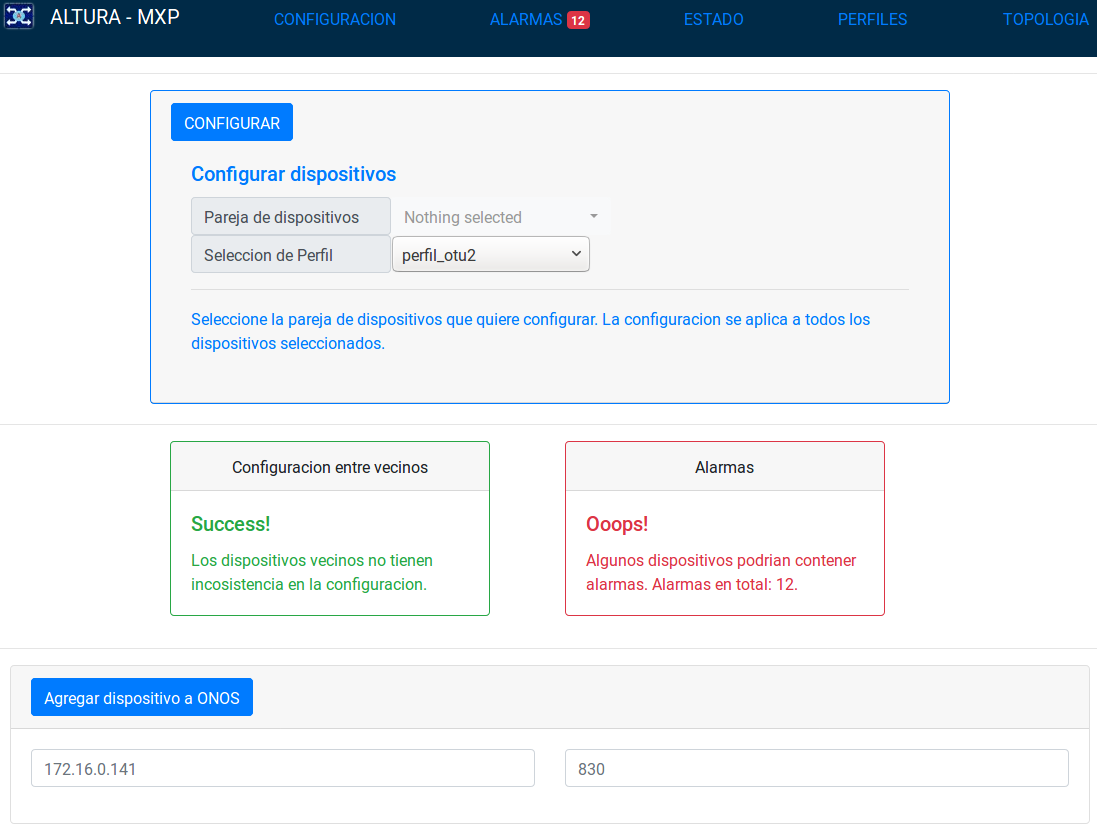
\includegraphics{Figures/test9_3.png}}
        \caption{Detección de configuración consistente entre dispositivos vecinos.}
        \label{fig:test9_3}
      \end{figure}

      Por último, se realiza nuevamente la prueba de conectividad realizando un ping entre los \textit{hosts}. Como se puede ver en la figura \ref{fig:test9_4}, los clientes ahora tienen conectividad entre ellos debido a la configuración consistente entre los dispositivos vecinos.

      \begin{figure}[H]
        \centering
        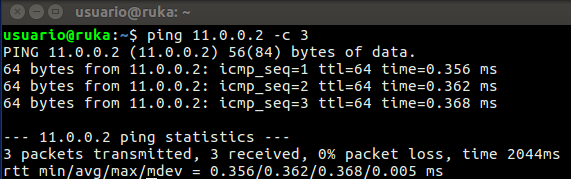
\includegraphics[scale=0.7]{Figures/test9_4.png}
        \caption{Prueba exitosa de conectividad entre \textit{host} A y \textit{host} B.}
        \label{fig:test9_4}
      \end{figure}
